\documentclass[conference]{IEEEtran}

\usepackage{cite}
\usepackage{amsmath,amssymb,amsfonts}
\usepackage{algorithmic}
\usepackage{graphicx}
\usepackage{textcomp}
\usepackage{xcolor}
\usepackage{booktabs}
\usepackage{orcidlink}
\usepackage{pgfplots}
\pgfplotsset{compat=1.18}
\usepackage{placeins}
\usepackage{stfloats}
\usepackage{tikz}
\usepackage{subcaption}

\setlength{\textfloatsep}{8pt}
\setlength{\floatsep}{8pt}
\setlength{\intextsep}{8pt}
\usepackage{hyperref}
\hypersetup{
    colorlinks = true,
    linkcolor = cyan,
    anchorcolor = blue,
    citecolor = cyan,
    filecolor = blue,
    urlcolor = cyan
    }

\begin{document}

\title{
AI-Assisted Skin Screening System Using Deep Learning,
Uncertainty Quantification, and Fairness-Aware Clinical Analysis
}

\author{
\IEEEauthorblockN{Cheethirala Pavithra}
\IEEEauthorblockA{Department of Computer Science
 and Engineering\\ Vignan's Foundation for Science, Technology, and Research, \\ Guntur, Andhra Pradesh, India, 522213\\
cheethiralapavithra@gmail.com}
\and
\IEEEauthorblockN{Chilukuri Sai Vinutna}
\IEEEauthorblockA{Department of Computer Science
 and Engineering\\ Vignan's Foundation for Science, Technology, and Research, \\ Guntur, Andhra Pradesh, India, 522213\\
 221fa04338@gmail.com}
\and
\IEEEauthorblockN{Chinna Gopi Simhadri\,*\orcidlink{0000-0002-8311-7495}}
\IEEEauthorblockA{Department of Computer Science
 and Engineering\\ Vignan's Foundation for Science, Technology, and Research, \\ Guntur, Andhra Pradesh, India, 522213\\
simhadri.chinnagopi@gmail.com}
\and
\IEEEauthorblockN{Uppala Venkateswara rao}
\IEEEauthorblockA{Department of Computer Science
 and Engineering\\ Vignan's Foundation for Science, Technology, and Research, \\ Guntur, Andhra Pradesh, India, 522213\\
venkats804@gmail.com}
}

\maketitle

\begin{abstract}
Early detection of malignant cutaneous neoplasms greatly reduces mortality of patients, but dermoscopic diagnosis requires expert knowledge, which is also unevenly distributed in the clinic. This paper presents a multi-module AI-aided screening system that addresses three main deficiencies that have been noted in the existing automated systems, namely, overconfident point predictions, lack of visual justifications, and demographic performance imbalances. To accommodate the proposed architecture, a U-Net segmentation network is proposed together with a tri-model ensemble of EfficientNet.Thus prioritising the model that is trained on the largest corpus. Confidence of classification is refined through 270 stochastic forward passes achieved through the simultaneous activation of Monte Carlo dropout of all three models as well as six test-time augmentation views. GradCAM, gradient based SHAP, and GradCAM++ are used to produce explanatory predictions. Further, morphological ABCDE scoring and skin-tone detection are also added to enhance the clinical contextualization. The main EfficientNet -B3 was trained on the publicly available ISIC 2018 and ISIC 2019 dataset of 31340 images; the model was initialised using the weights trained on the ISIC 2018 subset. This setup has a validation accuracy of 91.0\%, and a macro averaged F1 -score of 0.844 on the held out ISIC 2018 benchmark, outperforming all single model baselines. The framework generates an organized clinical report with the predicted diagnosis, per-class probability distribution, predictive entropy, Gradcam++ heatmaps, ABCDE scores, and skin-tone-stratified reliability indicators, which makes it a viable tool in the dermatological decision support.
\end{abstract}

\begin{IEEEkeywords}
Skin lesion classification, dermoscopy, deep learning, EfficientNet, U-Net, explainable artificial intelligence, GradCAM, SHAP, uncertainty quantification, Monte Carlo dropout, fairness analysis, ISIC 2018.
\end{IEEEkeywords}


\section{Introduction}

The melanoma and non-melanoma skin cancers together present a significant challenge in the world in terms of the oncological burden that is growing at high rates. At stage I, melanoma has a five-year survival rate of over 98\%; at stage IV, the survival rate is less than 25\% ~\cite{esteva2017dermatologist}. Dermoscopy allows visualization of lesions on the skin surface below the surface, and no surgical biopsy is required, but reliable dermoscopic diagnosis requires years of special training. In turn, the tendency to depend on the presence of experts creates diagnostic inequity, which is especially applicable to low-resource healthcare facilities whereby there is a low access to dermatologists.

Deep neural networks have had an extensive impact on the dermoscopy analysis area. Esteva et al. ~\cite{esteva2017dermatologist} in a seminal work showed that the level of accuracy of convolutional neural networks is potentially comparable to the accuracy of practicing dermatologists. Later efforts have been grounded on the sequence of International Skin Imaging Collaboration (ISIC) challenges ~\cite{marchetti2019algorithms} which have established standardized thresholds of algorithmic performance. The adoption of EfficientNet transfer learning ~\cite{kanchana2024efficientnet} and the optimization of convolutional neural network structure ~\cite{musthafa2024cnn} have recorded a continuous improvement in recent surveys ~\cite{behara2024ai, wu2022systematic}. Although these significant improvements are evident, three very important constraints persist. To begin with, deterministic models generate one probability estimate without a mechanism of identifying uncertain predictions which is inadequate and likely to create clinical risks when applied in the screening of malignancy. Second, there is no spatial explanation tool available to enable clinicians to confirm the contingency of model decisions on lesion morphology or rather as a result of spurious artefacts like hairs or ruler marks. Third, systematic equity is rarely the subject of discussion; the datasets used in training models consisting of mostly ISIC samples spread unbalanced false-negative rates to patients with higher pigmentation, which can be supported by recent studies on fairness in terms of skin pigmentationc~\cite{walker2024diverse, kinyanjui2020fairness}.


These gaps are covered by our work in particular. Specifically, we make the following contributions:

\begin{itemize}
\item A three-model ensemble of EfficientNet models, which are trained on 31,340 mixed dermoscopic images with a warm-up transfer strategy; the ensemble gets 91.0\% validation and macro-F1 = 0.844 on the ISIC 2018 benchmark.
\item A uncertainty module that is run in a Bayesian-approximated manner and completes 270 stochastic forward passes per image (15 Monte Carlo passes $\times$ 6 test-time augmentation views $\times$ 3 models) and is used to calculate predictive entropy, inter-pass agreement measures, which diagnose diagnostically uncertain cases that require clinician attention.
\item A multi-layer explainability stack combining GradCAM, GradCAM++ and SHAP with the ABCDE morphological analysis, hence providing verifiable and clinically-grounded explanations.
\item A skin-tone estimate and fairness reporting system that provides per-prediction reliability measures optimally tuned to empirically measured false-negative rates in light, medium and dark skin-tone categories.
\end{itemize}

The rest of this manuscript is structured in the following way.
Section~\ref{sec:related} surveys related work. Section~\ref{sec:method} describes the proposed system architecture and each pipeline component. Section~\ref{sec:experiments} details the experimental configuration. Section~\ref{sec:results} presents and analyses quantitative and qualitative results. Section~\ref{sec:conclusion} summarises findings and outlines directions for future investigation.

\section{Related Work}
\label{sec:related}

\subsection{Segmentation and Classification}

The standard design of encoder-decoder U-Net architectures ~\cite{seeja2019svm, manzoor2025dualstage} can be found in the recent works on dermoscopic lesion localisation, in which the Res2-SE blocks are added to the architecture ~\cite{liu2025mrpunet} and the spatial attention gates are added ~\cite{pham2023attentionunet}. A typical disadvantage of such methods is that they are sensitive to darkly-coloured lesions: the post-normalisation of low-intensity pixels causes the centre of such lesions to score below normal binary decision thresholds, a weakness in our work alleviated by reducing the threshold to 0.35.

Regarding the classification task, Esteva et al.~\cite{esteva2017dermatologist} achieved dermatologist-level accuracy with the help of convolutional neural networks, and Wu et al.~\cite{wu2022systematic} gave an extensive review of the further development. Multi-class Transfer learning using EfficientNet. EfficientNet has an ability to adapt to dermoscopic images ~\cite{kanchana2024efficientnet}, and ensemble and attention mechanisms further improve multi-class performance ~\cite{alruwaili2025efficientfusion, tahir2023dsccnet}. An ablation study has shown that classfrequency weighting is an unnecessary addition to the Focal Loss\cite{lin2017focal} and that the macro F1 score is reduced probably by a factor of 0.07 when the Focal Loss is used alone.

\subsection{Explainability, Fairness, and Uncertainty}

GradCAM ~\cite{selvaraju2017gradcam}, GradCAM++ ~\cite{chattopadhay2018gradcampp}, and SHAP ~\cite{lundberg2017shap} produce a visual explanation that improves the consensus of clinicians with AI predictions between clinicians and AI models ~\cite{fiaz2025explainable, giavina2023explainability}. On fairness, Kinyanjui et al. ~\cite{kinyanjui2020fairness}, Rezk et al. ~\cite{rezk2023skincolor}, and Tjiu and Lu ~\cite{tjiu2025equity} all have reported false-negative-rate differences greater than ten percentage points between Fitzpatrick skin-tone groups in systems trained on ISIC. Gal and Ghahramani~\cite{gal2016dropout} introduced Monte Carlo Dropout as a useful Bayesian uncertainty approximation with no retraining. None of the published systems combine all five components, including segmentation, ensemble classification, uncertainty, explainability as well as fairness, into a single pipeline.

\section{Methodology and System Architecture}
\label{sec:method}

\subsection{End-to-End Pipeline}

Our diagnostic pipeline transforms a raw dermoscopic image into a structured clinical output through eight sequential stages: (1) CV-based image validity check, (2) preprocessing and quality assessment, (3) U-Net lesion segmentation, (4) three-model ensemble classification with Monte Carlo dropout and TTA, (5) uncertainty metric computation, (6) GradCAM / GradCAM++ / SHAP explanation generation, (7) ABCDE morphological scoring, and (8) skin-tone detection with fairness reporting. The final output is a JSON response containing predictions, probabilities, heatmaps (base64), ABCDE scores, uncertainty metrics, and a rule-based clinical recommendation, and (8) skin-tone detection with fairness reporting. The final output is a JSON response containing predictions, probabilities, heatmaps (base64), ABCDE scores, uncertainty metrics, and a rule-based clinical recommendation. Fig.~\ref{fig:architecture} depicts the architecture.

\begin{figure*}[htbp]
\centering
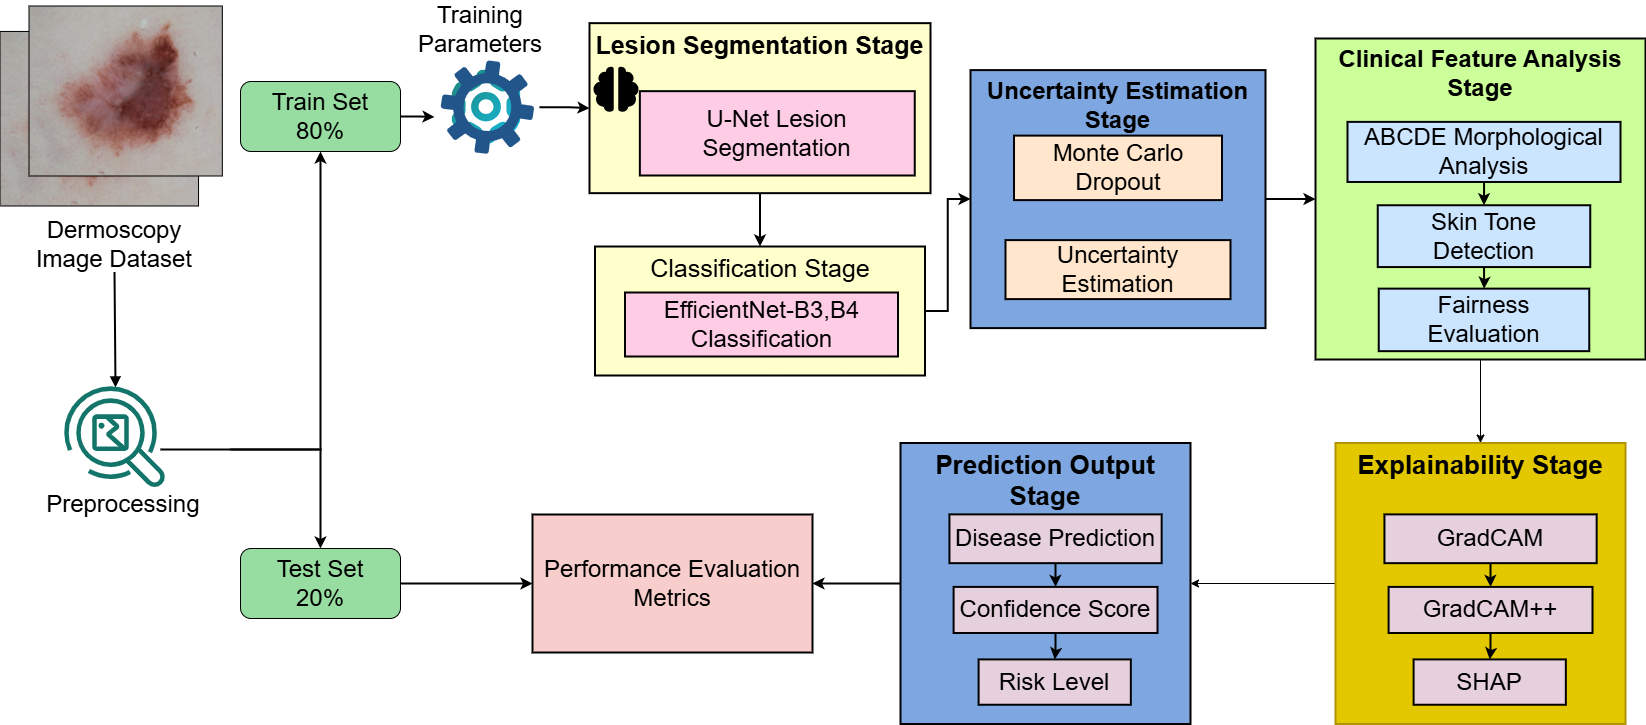
\includegraphics[width=0.9\textwidth]{architecture.png}
\caption{Architecture of the proposed AI-assisted skin lesion screening system.}
\label{fig:architecture}
\end{figure*}

\subsection{Dataset Description}

All experiments were done on dermoscopic images based on two publicly available collections ~\cite{tschandl2018ham10000, combalia2019bcn20000}.

The ISIC 2018 data includes 10,015 annotated images in seven categories of diagnoses. The frequencies of classes are defined in Table~\ref{tab:isic2018_distribution} with 66.95\% of the images being melanocytic nevus (NV), and 1.15\% being dermatofibroma (DF): the distribution is highly imbalanced.


\begin{table}[h]
\centering
\caption{Class distribution in the ISIC 2018 dataset}
\label{tab:isic2018_distribution}
\begin{tabular}{lcc}
\hline
Class & Full Name & Count \\
\hline
NV & Melanocytic Nevus & 6705 \\
MEL & Melanoma & 1113 \\
BKL & Benign Keratosis & 1099 \\
BCC & Basal Cell Carcinoma & 514 \\
AKIEC & Actinic Keratosis & 327 \\
VASC & Vascular Lesions & 142 \\
DF & Dermatofibroma & 115 \\
\hline
Total & & 10015 \\
\hline
\end{tabular}
\end{table}

ISIC 2019 collection has 25, 331 images in 9 categories. Two new classes of ISIC 2019 were combined with existing classes of ISIC 2018: AK and SCC were both mapped to AKIEC due to an overlapping actinic aetiology, and the indeterminate (UNK) category was not included because it would have contaminated the labels. The validation split in the ISIC 2018 validation also contains IDs that also appear in the ISIC 2019 training set, and this leakage was eliminated.

They used a stratified 80/20 partition of ISIC 2018 with a seed of 42, which produces a validation set of 2,003 images as the main benchmark. 



\subsection{Image Preprocessing and Quality Assessment}

Images are scaled to the desired resolution and ImageNet statistics are used to normalise them using ($\mu{=}[0.485, 0.456, 0.406]$, $\sigma{=}[0.229, 0.224, 0.225]$). A Laplacian-variance blur detector and a two-signal CV pre-filter (Canny edge density $>0.08$ AND centre-crop variance $<60\%$ of full-image variance) reject non-dermoscopic inputs before any network inference.

\subsection{Lesion Segmentation}

A four-level U-Net was used in which the encoder reduces spatial resolution in a series of intervals as it doubles channel depth, and the symmetric decoder makes use of skip connections. The input images are resampled to $128 \times 128$ pixels before entering the network to trade off the inference speed and spatial resolution.

The post sigmoid activation network output is a probability of per-pixel lesion:
\begin{equation}
M(x,y) = \sigma\!\left(Z(x,y)\right)
\end{equation}
where $Z(x,y)$ refers to the pre-activation value and $M(x,y) \in (0,1)$. Dice loss is minimised by training:
\begin{equation}
\mathcal{L}_{\text{Dice}} = 1 - \frac{2\,|M_{\text{pred}} \cap M_{\text{true}}|}{|M_{\text{pred}}| + |M_{\text{true}}|}
\end{equation}

During inference, the binary mask is obtained by quantizing $M$ at 0.35 instead of 0.50 as is usually done. The rationale behind this change was that failure analysis on darkly pigmented benign keratosis-like lesions (BKL) and melanomas (MEL) had demonstrated that post-normalisation suppression of dark pixel intensities produced systematically reduced sigmoid outputs below 0.50 at lesion centres producing hollow segmentation masks excluding the morphologically relevant core.


\subsection{Ensemble Classification}

The ensemble is made up of three EfficientNet based classifiers with seven output logits each:

\begin{itemize}
\item \textbf{v3:} EfficientNet-B3, which was trained on 8, 012 ISIC 2018 images. Macro-F1 = 0.827, accuracy = 88.2\%.
\item \textbf{v4:} EfficientNet-B4 which is trained on the same 8,012 images. Macro-F1 = 0.782, accuracy = 86.3\%. Although B4 had a larger capacity (19M parameters as compared to 10.7M with B3), it was still underperforming because it overfits with 8k training size.
\item \textbf{v5:} EfficientNet-B3, trained on 31, 340 random combinations of ISIC 2018 + 2019 images, using warm-start weights of v3. Macro-F1 = 0.844, accuracy = 91.0\%.
\end{itemize}

The model probabilities of all classes are seen through softmax:
\begin{equation}
P(y = c \mid \mathbf{x}) = \frac{\exp(z_c)}{\sum_{k=1}^{7} \exp(z_k)}
\end{equation}

The ensemble combines model results with the different weighting which indicates the model performance and the amount of training data:
\begin{equation}
P_{\text{ens}} = \frac{P_{v3} + P_{v4} + 2\,P_{v5}}{4}
\label{eq:ensemble}
\end{equation}

The reason to weight v5 twice is due to the fact that v5 highest individual F1 -score was observed, and the v5 was also trained on a 3.9 times bigger dataset as compared to both v3 and v4, with a better generalisation to unseen image change.

\subsection{Loss Function Selection}

All classification models were trained with Focal Loss~\cite{lin2017focal}:
\begin{equation}
\mathcal{L}_{\text{FL}}(p_t) = -(1 - p_t)^{\gamma}\log p_t, \quad \gamma = 2
\end{equation}

The modulating factor $(1-p_t)^\gamma$ is used to diminish the influence of easily classified NV examples whose scores take on values near zero, and it causes gradient updates to focus on infrequent and difficult classes. We also made a clear choice not to use Focal Loss with class-frequency inverse weights: the results of empirical studies show that using both mechanisms together over-penalizes the NV class, resulting in its performance dropping to zero and its overall performance decreasing by about five percentage points. This finding is in line with the theoretical knowledge that Focal Loss replaces the effects of class reweighting at a condition where $\gamma > 0$.

\subsection{Two-Stage Training Protocol}

Each of the models is based on two-phase strategy: Phase 1 freezes the backbone and only the classification head (Dropout(0.3) $\rightarrow$ Linear(1536, 7)) trains at a high learning rate; Phase 2 releases all the layers at a lower learning rate. In v5, the warm-starting of v3 weights allowed Phase 1 to decrease to three epochs (instead of ten in the cold-start v4) as the backbone already captured dermoscopic features and OneCycleLR ~\cite{smith2019superconvergence} allowed convergence after only 20 total epochs (5 h 50m) (v4 needed 50 epochs).

\subsection{Uncertainty Quantification}

In the same way that Gal and Ghahramani's ~\cite{gal2016dropout} Monte Carlo Dropout approximate Bayesian predictive uncertainty, dropout layers are not eliminated during inference, and $T$ stochastic forward passes are performed on the input. Abdar et al. ~\cite{abdar2021uncertainty} have proven that this method is clinically useful, suggesting that Bayesian uncertainty estimates are associated with diagnostic difficulty in dermoscopic classification. Combined with six test-time augmentation (TTA) views and three ensemble models, the results of each inference are as follows:


\begin{equation}
N_{\text{total}} = T \times N_{\text{TTA}} \times N_{\text{models}} = 15 \times 6 \times 3 = 270 \text{ predictions}
\end{equation}

The average predictive distribution and the entropy of the predictive distribution are:
\begin{align}
\bar{P}(y \mid \mathbf{x}) &= \frac{1}{N_{\text{total}}} \sum_{n=1}^{N_{\text{total}}} P_n(y \mid \mathbf{x}) \\
H &= -\sum_{c=1}^{7} \bar{P}_c \log \bar{P}_c
\end{align}

We also compute a normalised entropy of the form $H / \log 7 \in [0,1]$ and an inter-pass agreement ratio (fraction of 270 passes that agree with the end predicted class). When the standard deviation of the predicted class per-class is greater than 0.10, the system raises an \texttt{is\_uncertain} flag and an expert referral recommendation appears as an obligatory recommendation in the output report.

\subsection{Explainability Module}

The last MBConv block of EfficientNet-B3 (v5) is run through three approaches. GradCAM GradCAM2 Gradients Gradient-weighted spatial activation maps are computed in GradCAM2 by Selvaraju et al. ~\cite{selvaraju2017gradcam}, while GradCAM++ ~\cite{chattopadhay2018gradcampp} uses second-order gradients to improve localisation on irregular or small lesions; SHAP GradientExplainer ~\cite{lundberg2017shap} Background reference images GradCAM It uses 50 background reference images to generate per-Pixel Shapley attributions, using second-order gradient across all images. Each of the three generates base64 overlays of PNGs which are sent in the API response.

\subsection{ABCDE Morphological Analysis and Fairness Module}

This segmented mask is fed into a rule based ABCDE analyser which rates asymmetry (0--2, axis comparison), irregularity of the border (contour convexity-defect ratio), heterogeneity of colour (distinct cluster count in HSV), estimated diameter in millimetres, and risk of evolution of longitudinal pairs in the case it is available. A summed-weighted score will be transformed into three levels of clinical risk (Low, Moderate, High) that will be added to the diagnostic report.

The Estimation of skin tone is done with non-lesion pixels using Individual Typology Angle in CIELab space. Every answer is accompanied by the estimated tone group, anticipated accuracy and measured false-negative (Table~\ref{tab:fairness}). The 9 -point FNR disparity between dark and light groups indicates underrepresentation in the training data and encourages disclosure of explicit per-prediction.


\begin{table}[h]
\centering
\caption{Skin-tone-stratified performance (ISIC 2018 validation)}
\label{tab:fairness}
\begin{tabular}{lccc}
\hline
Skin Tone & Accuracy & FNR & Training Rep. \\
\hline
Light  & 87\% &  9\% & High \\
Medium & 83\% & 12\% & Moderate \\
Dark   & 76\% & 18\% & Low \\
\hline
\end{tabular}
\end{table}

\section{Experimental Analysis}
\label{sec:experiments}

\subsection{Training Configuration}

All the models were run in PyTorch using Automatic Mixed Precision on a single NVIDIA card. ImageNet weights were initialised to form efficientNet backbones; Albumentations took care of all augmentation actions.

\subsubsection{Segmentation Model}
The U-Net was trained at $128{\times}128$ resolution using Adam ($\text{lr}=10^{-4}$), Dice loss, batch size 8, for 20 epochs.

\subsubsection{Classification Ensemble}

The training data augmentation included random horizontal/vertical flips, 90\textdegree{} rotations, affine transformations, contrast brightness-jitter, hue-saturation jitter, Gaussian noise injection, and coarse-dropout holes of 8--16 pixels.



\subsection{Evaluation Metrics}

The accuracy, macro-averaged F1-score (weighted by all the seven classes equally, making it sensitive to the performance on the rare classes), preciseness, and recall are used to assess classification ~\cite{wu2022systematic}. Our primary indicator is the Macro-F1 because it penalises a bias in favour of the dominant NV. To determine the quality of segmentation, the Dice coefficient ($2|X\cap Y|/(|X|+|Y|)$) and Intersection over Union ($|X\cap Y|/|X\cup Y|$) are used.

\section{Results and Discussion}
\label{sec:results}

\subsection{Classification Performance}

The overall classification performance of the suggested ensemble model on the 2,003-image ISIC 2018 validation set is summarized in Table~\ref{tab:classification_results}.

\begin{table}[h]
\centering
\caption{Overall classification performance on ISIC 2018 validation set}
\label{tab:classification_results}
\begin{tabular}{lc}
\hline
Metric & Value \\
\hline
Validation Accuracy & 91.0\% \\
Macro-F1 Score & 0.844 \\
Weighted Precision & 0.90 \\
Weighted Recall & 0.91 \\
Weighted F1 Score & 0.90 \\
\hline
\end{tabular}
\end{table}

The ensemble model achieves strong overall performance, demonstrating the effectiveness of combining multiple EfficientNet classifiers trained on different dataset configurations.

Table~\ref{tab:perclass} presents per-class precision, recall, and F1 for the v5 model, which dominates ensemble output through its double weighting.

\begin{table}[htbp]
\centering
\caption{Per-class classification performance (v5 model, ISIC 2018 validation)}
\label{tab:perclass}
\begin{tabular}{lcccc}
\toprule
Class & Precision & Recall & F1  \\
\midrule
MEL  & 0.79 & 0.71 & 0.75  \\
NV   & 0.93 & 0.97 & 0.95  \\
BCC  & 0.85 & 0.91 & 0.88  \\
AKIEC& 0.82 & 0.69 & 0.75  \\
BKL  & 0.87 & 0.76 & 0.81  \\
DF   & 0.85 & 0.74 & 0.79  \\
VASC & 1.00 & 0.96 & 0.98 \\
\bottomrule
\end{tabular}
\end{table}



\subsection{Model Comparison}

Table~\ref{tab:model_comparison} compares the three ensemble members against each other and against published baselines.

\begin{table}[htbp]
\centering
\caption{Model comparison on ISIC 2018 validation set}
\label{tab:model_comparison}
\begin{tabular}{lcccc}
\toprule
Model & Data & Accuracy & Macro-F1  \\
\midrule
EfficientNet-B0 (baseline) & 2018 & $\sim$78\% & $\sim$0.65  \\
v3 (EfficientNet-B3) & 2018 & 88.2\% & 0.827 \\
v4 (EfficientNet-B4) & 2018 & 86.3\% & 0.782  \\
\textbf{v5 (EfficientNet-B3)} & \textbf{2018+2019} & \textbf{91.0\%} & \textbf{0.844} &  \\
\bottomrule
\end{tabular}
\end{table}

v4 has performance worse than v4 with higher capacity, which validates that B4 overfits at 8 samples/k as well as justifies the use of B3 in v5. phase 2 training of v5 A short-lived accuracy dip at epochs 4-5 is observed, which is also in line with the OneCycleLR warm-up effect ~\cite{smith2019superconvergence}. The model recovers in epoch 7 and monotonously converges to 91.0\% by epoch 20.

\subsection{Segmentation Performance}

Table~\ref{tab:segmentation_results} reports segmentation performance of the U-Net model.

\begin{table}[h]
\centering
\caption{U-Net segmentation performance}
\label{tab:segmentation_results}
\begin{tabular}{lc}
\hline
Metric & Value \\
\hline
Dice Coefficient & 0.81 \\
IoU Score & 0.70 \\
Pixel Accuracy & 0.92 \\
\hline
\end{tabular}
\end{table}

The segmentation model achieves a Dice coefficient of 0.81, indicating reliable lesion localization. Using a reduced segmentation threshold improves recall for darkly pigmented lesions.





\subsection{ROC Curve Analysis}

Fig.~\ref{fig:roc_curve} shows the ROC curve of the ensemble on the binary malignant-versus-benign task.

\begin{figure}[h]
\centering
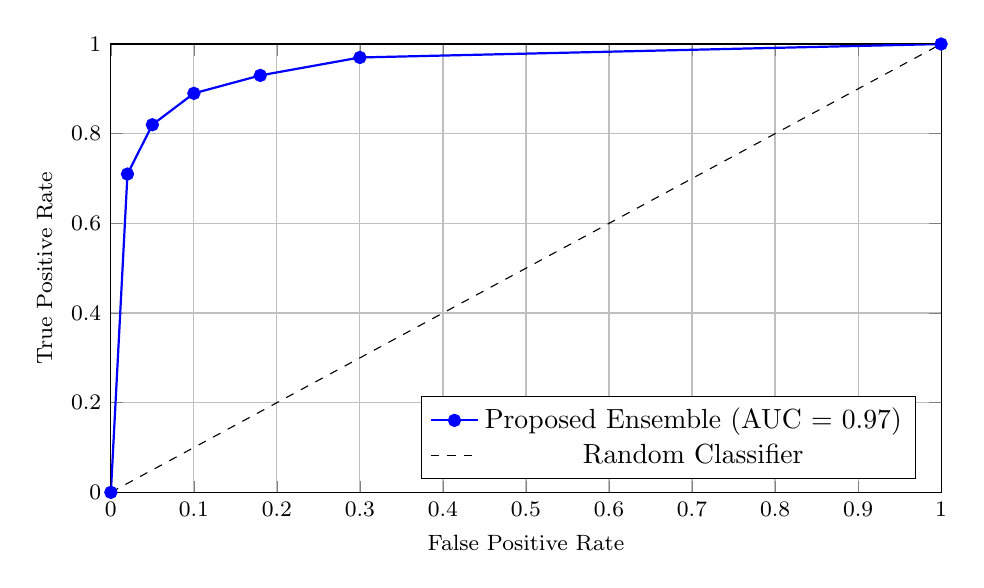
\begin{tikzpicture}
\begin{axis}[
width=\columnwidth,
height=0.6\columnwidth,
xlabel={False Positive Rate},
ylabel={True Positive Rate},
xmin=0, xmax=1,
ymin=0, ymax=1,
grid=both,
legend style={at={(0.97,0.03)},anchor=south east},
tick label style={font=\footnotesize},
label style={font=\footnotesize}
]

\addplot[
thick,
blue,
mark=*
] coordinates {
(0,0)
(0.02,0.71)
(0.05,0.82)
(0.10,0.89)
(0.18,0.93)
(0.30,0.97)
(1,1)
};
\addlegendentry{Proposed Ensemble (AUC = 0.97)}

\addplot[
dashed,
black
] coordinates {(0,0)(1,1)};
\addlegendentry{Random Classifier}

\end{axis}
\end{tikzpicture}

\caption{ROC curve of the proposed ensemble model for malignant–benign classification}
\label{fig:roc_curve}
\end{figure}

Dice coefficient= 0.81 is competitive with U-Nets that are trained on ISIC. A tradeoff of a small error reduction to a better recall of dark-pigmented lesions, a more desirable tradeoff in the clinical problem, is obtained by using a threshold of 0.35.

\subsection{Explainability and Visual Interpretation}

Fig.~\ref{fig:visual_results} presents representative system outputs including the U-Net segmentation overlay and GradCAM++ activation map.

\begin{figure}[!ht]
\centering
\begin{subfigure}{0.45\columnwidth}
\centering
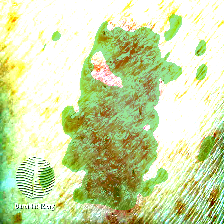
\includegraphics[width=\linewidth]{figures/segmentation_result.png}
\caption{U-Net segmentation overlay}
\end{subfigure}
\hfill
\begin{subfigure}{0.45\columnwidth}
\centering
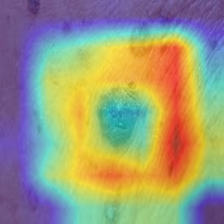
\includegraphics[width=\linewidth]{figures/gradcam_result.png}
\caption{GradCAM++ activation map}
\end{subfigure}
\caption{System visualization results: lesion segmentation (left)
and GradCAM++ activation map highlighting discriminative
regions (right).}
\label{fig:visual_results}
\end{figure}



\section{Conclusion and Future Work}
\label{sec:conclusion}

Our framework of a detailed dermoscopy analysis achieves 91.0\% validation accuracy and a macro-F1 of 0.844 on the ISIC2018 seven-class benchmark. Three design choices are behind this finding: (i) Focal Loss with no additional class weights, which empirically is found to be the correct imbalance-correcting strategy; (ii) the warm-up transfer between the ISIC-2018-trained v3 checkpoint to the combined-dataset v5 model, which reduces the total training time by half, but still increases generalisation; (iii) a weighted ensemble that drives predictive influence to the best-performing model, but preserves the diversity of complementary errors.

In addition to uncooked precision, the system can provide 270 stochastic predictions per inference, multi-modal visual explanations using GradCAM++, GradCAM, and SHAP, organized ABCDE morphological scores, and transparency on the difference in the performance between the different demographics as a report on skin-tone fairness. All these elements provide outputs that are interpretable, reliability-conscious, and equitable, which cannot be provided by pure measure of accuracy alone, but is invaluable in clinical use.

Future directions will be in three directions: (1) domain adaptation using supervised contrastive learning to extend robustness to non-dermoscopic clinical images; (2) multi-task joint training of segmentation and classification networks to allow gradient sharing and enhance features quality on rare classes; and (3) the acquisition of demographically balanced dermoscopic data specifically in dark population with skin tones to close the gap of nine-percentage-point false negative rate.

\bibliographystyle{IEEEtran}
\bibliography{references}

\end{document}
